%%%%%%%%%%%%%%%%%%%%%%%%%%%%%%%%%%%%%%%%%%%%%%%%%%%%%%%%%%%%%%%%%%%%%%
% Source: Dave Richeson (divisbyzero.com), Dickinson College
% 
% A one-size-fits-all LaTeX cheat sheet. Kept to two pages, so it 
% can be printed (double-sided) on one piece of paper
% 
% Feel free to distribute this example, but please keep the referral
% to divisbyzero.com
% 
% If you're new to LaTeX, the wikibook is a great place to start:
% http://en.wikibooks.org/wiki/LaTeX
%%%%%%%%%%%%%%%%%%%%%%%%%%%%%%%%%%%%%%%%%%%%%%%%%%%%%%%%%%%%%%%%%%%%%%

\documentclass[10pt,landscape]{article}
\usepackage{amssymb,amsmath,amsthm,amsfonts}
\usepackage{multicol,multirow}
\usepackage{calc}
\usepackage{ifthen}
\usepackage{bm}
\usepackage[landscape]{geometry}
\usepackage[colorlinks=true,citecolor=blue,linkcolor=blue]{hyperref}
\usepackage{graphicx}
\graphicspath{{./images/}}

\ifthenelse{\lengthtest { \paperwidth = 11in}}
    { \geometry{top=0.1in,left=0.1in,right=0.1in,bottom=0.1in} }
	{\ifthenelse{ \lengthtest{ \paperwidth = 297mm}}
		{\geometry{top=0.1cm,left=0.1cm,right=0.1cm,bottom=0.1cm} }
		{\geometry{top=0.1cm,left=0.1cm,right=0.1cm,bottom=0.1cm} }
	}
\pagestyle{plain}
\makeatletter
\renewcommand{\section}{\@startsection{section}{1}{0mm}%
                                {-1ex plus -.5ex minus -.2ex}%
                                {0.5ex plus .2ex}%x
                                {\normalfont\large\bfseries}}
\renewcommand{\subsection}{\@startsection{subsection}{2}{0mm}%
                                {-1explus -.5ex minus -.2ex}%
                                {0.5ex plus .2ex}%
                                {\normalfont\normalsize\bfseries}}
\renewcommand{\subsubsection}{\@startsection{subsubsection}{3}{0mm}%
                                {-1ex plus -.5ex minus -.2ex}%
                                {1ex plus .2ex}%
                                {\normalfont\small\bfseries}}                       
\makeatother
\setcounter{secnumdepth}{0}
\setlength{\parindent}{0pt}
\setlength{\parskip}{0pt plus 0.5ex}
% -----------------------------------------------------------------------

\title{MA2108 Finals Cheatsheet}

\begin{document}

\raggedright
%\footnotesize
\scriptsize

\begin{center}
     \Large{\textbf{NUS MA2108 Finals Cheatsheet}} \\
\end{center}
\begin{multicols}{4}
\setlength{\premulticols}{1pt}
\setlength{\postmulticols}{1pt}
\setlength{\multicolsep}{1pt}
\setlength{\columnsep}{1pt}

% \section{Preliminaries}
% \subsection{Sets}
% \textbf{Theorem 1.1.4} If $A, B, C$ are sets, then

% (a) $A \backslash (B \cup C) = (A \backslash B) \cap (A \backslash C)$,

% (b) $A \backslash (B \cap C)$ = $(A \backslash B) \cup (A \backslash C)$

% \subsection{Functions}
% \textbf{Definition 1.1.6} 

% The set $A$ is called the domain of $f$ and is often denoted by $D(f)$.

% The set $B$ is called the codomain of $f$.

% The set $f(A) = \{ f(x) : x \in A \}$ is called the range of $f$, denoted by $R(f).$ Note that although $D(f) = A$, we only have $R(f) \subseteq B$.

% \textbf{Definition 1.1.7} If $E$ is a subset of $A$, then the \textbf{direct image} of $E$ under $f$ is the subset $f(E)$ of $B$ given by 

% $$
% f(E) := \{ f(x): x \in E \}
% $$

% If $H$ is a subset of $B$, then the \textbf{inverse image} of $H$ under $f$ is the subset $f^{-1}(H)$ of $A$ given by 

% $$
% f^{-1}(H) := \{ x \in A: f(x) \in H \}
% $$

% \textbf{Definition 1.1.9} Let $f: A \mapsto B$ be a function from $A$ to $B$.

% (a) The function $f$ is said to be \textbf{injective} (or \textbf{one-one} if whenever $x_1 \neq x_2$, then $f(x_1) \neq f(x_2)$. 

% (b) The function is said to be \textbf{surjective} (or to map $A$ \textbf{onto} $B$) if $R(A) = B$. 

% (c) if $f$ is both injective and surjective, then $f$ is said to be \textbf{bijective}.

% \textbf{Definition 1.1.11} Let $f: A \mapsto B$ be a bijection of $A$ onto $B$. Then the \textbf{inverse function} $f^{-1}: B \mapsto A$ is defined such that $f^{-1}(f(x)) = x, \forall x \in A$ and $f(f^{-1}(y)) = y, \forall y \in B$.

% Note that $f^{-1}$ is also bijective by replacing $f$ with $f^{-1}$ in definition 1.1.11.

% \subsection{Mathematical Induction}
\textbf{Well-ordering principle for $\mathbb{N}$} Every non empty subset $S$ of $\mathbb{N}$ has a least element, i.e. there exists $m \in S$ such that $m \leq k, \forall k \in S$.

% \subsection{Finite and Infinite sets}
% \textbf{Definition 1.3.6} (a) A set $S$ is said to be \textbf{denumerable} (or \textbf{countably infinite}) if there exists a bijection of $\mathbb{N}$ onto $S$.

% (b) A set $S$ is said to be \textbf{countable} if it is either finite or denumerable

% (b) A set $S$ is said to be \textbf{uncountable} if it is not countable.

% \textbf{1.3.8 Theorem} The set $\mathbb{N \times N}$ is denumerable.

% \textbf{1.3.9 Theorem} Suppose that $S$ and $T$ are sets and that $T \subseteq S$.

% (a) If $S$ is a countable set, then $T$ is a countable set.

% (b) If $T$ is an uncountable set, then $S$ is an uncountable set.

% \textbf{1.3.10 Theorem} The following statements are equivalent:

% (a) $S$ is a countable set.

% (b) There exists a surjection of $\mathbb{N}$ onto $S$.

% (b) There exists an injection of $S$ onto $\mathbb{N}$.

% \textbf{1.3.11 Theorem} The set $\mathbb{Q}$ of all rational numbers is denumerable, that is, the set is capable of being assigned a bijection to the natural numbers.

% \textbf{1.3.12 Theorem} If $A_m$ is a countable set for each $m \in \mathbb{N}$, then the union $A:= \cup^{\infty}_{m=1} A_m$ is countable.

\section{The Real Numbers}
% \subsection{The Algebraic Property of $\mathbb{R}$}

% \subsection{Number Systems}
% $\mathbb{Z} = \{ 0, \pm 1, \pm 2, \cdots \}$ is the set of \textit{integers}.

% $\mathbb{Q} = \{ \frac{p}{q}: p, q \in \mathbb{Z}, q \neq 0 \} $ is the set of \textit{rational numbers}.

% $\mathbb{R}$ denotes the set of \textit{real numbers}.

% $\mathbb{C} = \{ x + iy: x, y \in \mathbb{R} \} $ is the set of \textit{complex numbers}.

% $\mathbb{Z} \subset \mathbb{Q} \subset \mathbb{R} \subset \mathbb{C}$

% \textbf{Theorem 2.1.4} There does not exist a rational number $r$ such that $r^2 = 2$ i.e. $\sqrt{2}$ is irrational $(\sqrt{2} \notin \mathbb{Q})$

% \subsection{Field}
% \textbf{Definition.} A \textit{field} $\mathbb{F, +, \times}$ is a set $\mathbb{F}$ together with two binary operations $+$ and $\times$ called \textit{addition} and \textit{multiplication} respectively satisfying the following axioms:

% \textbf{(A1)} (Closure for addition) For all $x, y \in \mathbb{F}, x + y \in \mathbb{F}$.

% \textbf{(A2)} (Addition is commutative) $x + y = y + x$ for all $x, y \in \mathbb{F}$.

% \textbf{(A3)} (Addition is associative) $(x + y) + z = x + (y + z)$ for all $x, y, z \in \mathbb{F}$.

% \textbf{(A4)} (Additive identity) There exists $0 \in \mathbb{F}$ st for all $x \in \mathbb{F}$, $x + 0 = x$.
% Note that (A4) defines $0$.

% \textbf{(A5)} (Additive inverse) For every $x \in \mathbb{F}$ there exists $y \in \mathbb{F}$ (y depends on x) such that $x + y = 0.$ We denote $y$ by $-x$.

% \textbf{(M1)} (Closure for multiplication) For all $x, y \in \mathbb{F}, x \times y \in \mathbb{F}$.

% \textbf{(M2)} (Multiplication is commutative) $x \times y = y \times x$ for all $x, y \in \mathbb{F}$.

% \textbf{(M3)} (Multiplication is associative) $(x \times y) \times z = x \times (y \times z)$ for all $x, y, z \in \mathbb{F}$.

% \textbf{(M4)} (Multiplicative identity) There exists $1 = 1_{\mathbb{F}} \in \mathbb{F}, 1 \neq 0$ such that for all $x \in \mathbb{F}$, $1 \times x = x$.
% Note that (A4) defines $1$.

% \textbf{(M5)} (Multiplicative inverse) For every nonzero $x \in \mathbb{F}$ there exists $y \in \mathbb{F}$ ($y$ depends on $x$) such that $x \times y = 1$. We call $y$ the multiplicative inverse of $x$ and we denote $y$ by $x^{-1}$.

% \textbf{(D)} (Distributive Law) $x \times (y + z) = (x \times y) + (x \times z)$ for all $x, y, z \in \mathbb{F}$.

% \textbf{Remark.} Axioms (A1)-(A5) says that $(\mathbb{F}, +)$ forms a \textit{commutative group}, and axioms (M1)-(M5) says that $(\mathbb{F} - \{ 0 \}, \times)$ forms another \textit{commutative group}. Axiom (D) connect the two group structures.

% Note that lecture slides did not include closure properties. Safer to write the axiom rather than abbreviation (eg (A1)).

% \textbf{Example.} The sets $\mathbb{R, C, Q}$ with the usual addition and multiplication is a field. However, $\mathbb{Z}$ is not a field.

% \textbf{Theorem} Let $\mathbb{F}$ be a field.

% If $a \in \mathbb{F}$, then $0a = 0$.

% If $a \in \mathbb{F}$, then $(-1)a = -a$.

% If $a, b \in \mathbb{F}$ and $ab = 0$, then \textit{either} $a = 0$ or $b = 0$.

\subsection{The Order Property of $\mathbb{R}$}
% \textbf{2.1.5 Axioms} Order properties of the positive real numbers of $\mathbb{R}$:

% (i) If $a$ and $b$ are positive, then $a + b$ are positive;

% (ii) If $a$ and $b$ are positive, then $ab$ are positive;

% (iii) (The Trichotomy property) For any $a \in \mathbb{R}$, then exactly one of the following properties holds:

% $$
% \text{$a$ is positive, $a = 0$, or $-a$ is positive}
% $$

% \textbf{Definition 2.1.6} Let $a, b$ be elements of $\mathbb{R}$.

% (a) If $a - b$ are positive, then we write $a > b$.

% (b) If $a - b$ are positive or 0, then we write $a \geq b$.

% The \textit{Trichotomy property} implies that if $a, b \in \mathbb{R}$, then exactly one of the following properties holds:

% $$
% a > b, \enskip a = b, \enskip or \enskip a < b
% $$

% \textbf{Theorem 2.1.7} Let $a, b, c$ be any elements of $\mathbb{R}$.

% (a) $a < b$ and $b < c \implies a < c$

% (b) $a < b \implies a + c < b + c, \forall c \in \mathbb{R}$

% (c) ($a < b$ and $c > 0 \implies ac < bc$) and ($a < b$ and $c < 0 \implies ac > bc$)

% We have a real number $a$ (i) positive ($a>0$), (ii) nonnegative ($a \geq 0$), (iii) negative ($a < 0$), (iv) nonpositive ($a \leq 0$). 

% \textbf{Theorem 2.1.8(a)} For any nonzero real number $a, a^2 > 0$

% \textbf{Theorem 2.1.9} If $a \in \mathbb{R}$ is such that $0 \leq a < \epsilon$ for \textbf{every} positive number $\epsilon$, then $a = 0$.

% \textbf{Theorem 2.1.10} If $ab > 0$, then either

% (i)  $a > 0$ and $b > 0$, or 

% (ii) $a < 0$ and $b < 0$

% \textbf{Corollary 2.1.11} If $ab < 0$, then either 

% (i)  $a < 0$ and $b > 0$, or 

% (ii) $a > 0$ and $b < 0$

\textbf{Bernoulli's Inequality} If $x > -1$, then $(1 + x)^n \geq 1 + nx, \forall n \in \mathbb{N}$.

% \textbf{Popular Means in MA/ST modules.} Let $n \geq 2$ and let $a_1, a_2, \cdots, a_n$ be positive numbers.

% (i) The \textbf{arithmetic mean} is defined as $A = \frac{a_1, a_2, \cdots, a_n}{n}$.

% (ii) The \textbf{geometric mean} is defined as $G = (a_1a_2 \cdots a_n)^{1/n}$.

% (iii) The \textbf{harmonic mean} is defined as $H = \frac{n}{\frac{1}{a_1} + \frac{1}{a_2} + \cdots + \frac{1}{a_n}}$.

% Remark that $H \leq G \leq A$.

\subsection{Absolute Value and the Real Line}
% \textbf{Definition 2.2.1} Let $a \in \mathbb{R}$. The \textbf{absolute value} of $a$ is defined by 

% $$
% |a|=\left\{\begin{array}{c}
% a \text { if } a>0 \\
% -a \text { if } a<0 \\
% 0 \text { if } a=0
% \end{array}\right.
% $$

% \textbf{Observation.}

% $|a| \geq 0, a \leq |a|$ and $-a \leq |a|, \forall a \in \mathbb{R}$

% $|-a| = |a|, \forall a \in \mathbb{R}$

% $|a| = 0 \iff a = 0$

\textbf{Theorem 2.2.2 (Properties of absolute value)}

(a) $|ab| = |a||b|, \forall a,b \in \mathbb{R}$

(b) $|a|^2 = a^2, \forall a \in \mathbb{R}$

(c) If $c \geq 0,$ then $|a| \leq c \iff -c \leq a \leq c$

(d) $-|a| \leq a \leq |a|, \forall a \in \mathbb{R}$

\textbf{Theorem 2.2.3 Triangle Inequality}  If $a, b \in \mathbb{R}$, then $|a + b| \leq |a| + |b|$

\textbf{Corollary 2.2.4} For $a, b \in \mathbb{R}$, one has

(i) $||a| - |b|| \leq |a - b| \equiv -|a - b| \leq |a| - |b| \leq |a - b|

(ii) $|a - b| \leq |a| + |b|$

\textbf{Corollary 2.2.5} If $a_1, a_2, \cdots, a_n$ are any real numbers, then 

$$
|a_1 + a_2 + \cdots + a_n| \leq |a_1| + |a_2| + \cdots + |a_n|
$$

\textbf{Definition 2.2.7} Let $a \in \mathbb{R}$ and $\epsilon > 0.$ Then the $\epsilon-$\textbf{neighborhood} of $a$ is the set $V_{\epsilon}(a) := \{ x \in \mathbb{R}: |x-a| < \epsilon \}$. 

% For $a \in \mathbb{R}$, the statement that $x$ belongs to $V_{\epsilon}(a)$ is equivalent to either of the statement $-\epsilon < x - a < \epsilon \equiv a - \epsilon < x < a + \epsilon$

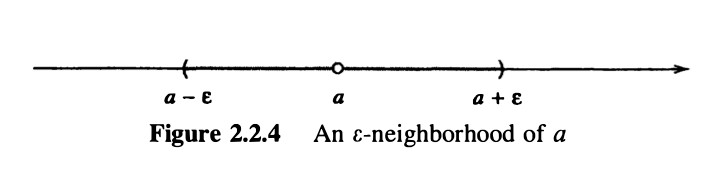
\includegraphics[width=\columnwidth]{images/d-2.2.7.png}

% \textbf{Theorem 2.2.8} Let $a \in \mathbb{R}$. If $x$ belongs to the neighbourhood $V_{\epsilon}(a)$ for every $\epsilon > 0$, then $x = a$. Alternatively, $\underset{\epsilon > 0}{\bigcap} V_{\epsilon}(a) = \{ a \}$.
 
\subsection{The Completeness Property of $\mathbb{R}$}
% \textbf{Definition 2.3.1}  Let $S$ be a nonempty subset of $\mathbb{R}$.

% (a) A number $u \in \mathbb{R}$ is called an \textbf{upper bound} of $S$ if $s \leq u, \forall s \in S$

% (b) A number $w \in \mathbb{R}$ is called a \textbf{lower bound} of $S$ if $w \leq s, \forall s \in S$.

% The idea of upper and lower bound is applied to functions by considering the range of a function. For example, given a function $f : D \mapsto \mathbb{R}$, $f$ is \textbf{bounded above} if $\exists B \in \mathbb{R} : f(x) \leq B, \forall x \in D$. \\

% \textbf{Definition 2.3.1} We say that a nonempty set $S \in \mathbb{R}$ is:

% (a) \textbf{bounded above} if $S$ has an upper bound

% (b) \textbf{bounded below} if $S$ has a lower bound

% (c) \textbf{bounded} if $S$ has an upper bound and a lower bound;

% (d) \textbf{unbounded} if $S$ is not bounded, that is, either it does not have any upper bound or it does not have any lower bound.

\textbf{Definition 2.3.2(a)} Let $S$ be a nonempty subset of $\mathbb{R}$. A number $u$ is said to be \textbf{supremum} (or least upper bound) of $S$ if it satisfies the conditions

(1) $u$ is an upper bound of $S$ (i.e. $s \leq u, \forall s \in S$). By defn of upper bound, $u \in \mathbb{R}$.

(2) if $v$ is any upper bound of $S$, then $u \leq v$.

% \textbf{Equivalent Definition, Lemma 2.3.3} Let $S$ be a nonempty subset of $\mathbb{R}$. A number $u$ is said to be \textbf{supremum} of $S$ if it satisfies the conditions

% (1) $u$ is an upper bound of $S$ (i.e. $s \leq u, \forall s \in S$). By defn of upper bound, $u \in \mathbb{R}$.

% (2) if $v < u$, then there exists $s' \in S$ st $v < s'$ (i.e. $v$ can not be an upper bound of $S$.)

\textbf{Definition 2.3.2(b)} Let $S$ be a nonempty subset of $\mathbb{R}$. A number $w$ is said to be \textbf{infimum} (or greatest lower bound) of $S$ if it satisfies the conditions:

(1) $w$ is an lower bound of $S$ (i.e. $w \leq s, \forall s \in S$). By defn of lower bound, $w \in \mathbb{R}$.

(2) if $t$ is any lower bound of $S$, then $t \leq w$.

% \textbf{Equivalent Definition} Let $S$ be a nonempty subset of $\mathbb{R}$. A number $w$  is said to be infimum (or greatest lower bound) of $S$ if it satisfies the conditions:

% (1) $w$ is a lower bound of $S$ (i.e. $w \leq s, \forall s \in S$). By defn of lower bound, $w \in \mathbb{R}$.

% (2) if $t > w$, then there exists $s' \in S$ st $s' < t$ (ie $t$ cannot be a lower bound of $S$).

% Note the following remarks on supremum and infimum

% (1) there can only be one supremum and infimum of a given subset $S$ of $\mathbb{R}$, denoted by $\sup S$ and $\inf S$

% (2) the supremum and infimum of a set \textbf{may or may not} be the elements of the set.

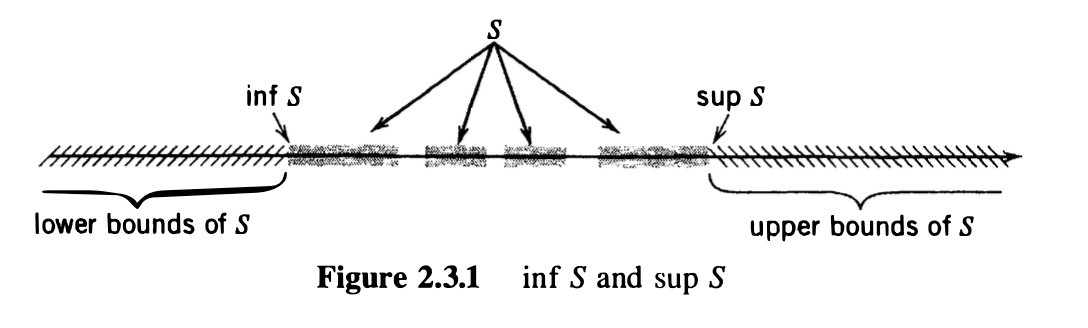
\includegraphics[width=\columnwidth]{images/inf-sup.png}

% \textbf{Terminologies} Let $S$ be a nonempty subset of $\mathbb{R}$.

% (i) If $u = \operatorname{\sup} S$ and $u \in S$, then $u$ is also called the \textbf{maximum} of $S$. In this case, we write $u = \operatorname{max} S$.

% (ii) If $w = \inf S$ and $w \in S$, then $w$ is also called the \textbf{minimum} of $S$. In this case, we write $w = \operatorname{min} S$.

% \textbf{Lemma 2.3.4} Let $u$ be an upper bound of $S \subset \mathbb{R}$. Then $u = \sup S \iff \forall \epsilon > 0, \exists s_{\epsilon} \in S: u - \epsilon < s_{\epsilon}$.

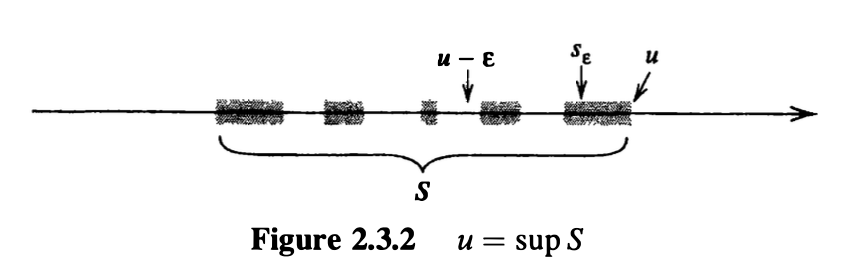
\includegraphics[width=\columnwidth]{images/u=supS.png}

\textbf{The Supremum/Infimum Property (Axiom) of $\mathbb{R}$} Every \textbf{nonempty} subset of $\mathbb{R}$ that has an upperbound/lowerbound has a supremum/infimum.

\subsection{Applications of the Supremum Property}

\textbf{2.4.3 Archimedean Property} If $x \in \mathbb{R}$, then $\exists n_x \in \mathbb{N}: x < n_x$. 

% \textbf{Corollary 2.4.4} Let $S = \{ \frac{1}{n} : n \in \mathbb{N} \} = \{ 1, \frac{1}{2}, \frac{1}{3}, \cdots \} $. Prove that $\inf S = 0$.

\textbf{Corollary 2.4.5} For any $\epsilon > 0$, $\exists n \in \mathbb{N} : \frac{1}{n} < \epsilon$. Note that the numerator can be any constant $c \in \mathbb{N}$. Let $n' := cn \in \mathbb{N}.$

$$
\frac{c}{n'} < \epsilon \iff \frac{1}{n} < \epsilon
$$

% \textbf{Corollary 2.4.6} If $x > 0$, then $\exists n \in \mathbb{N}: n - 1 \leq x < n$.

% \textbf{Theorem 2.4.7} There exists a unique positive real number $b$ with $b^2 = 2$.

\textbf{Theorem 2.4.8 (The Density Theorem of $\mathbb{Q}$)} If $x, y \in \mathbb{R}$ with $x < y$, then there exists a rational number $r \in \mathbb{Q} : x < r < y$.

\textbf{Corollary (The Density Theorem of Irrational Numbers)} If $x, y \in \mathbb{R}$ with $x < y$, then there exists an irrational number $z : x < z < y$.

% \subsection{Examples for the Supremum Property.}

% \textbf{W5P15} $\sup \{-x_n : n \in \mathbb{N} \} = - \inf \{ x_n: n \in \mathbb{N} \}$

% \textbf{Example 2.4.1(a)} Let $S$ be a nonempty subset of $\mathbb{R}$ that is bounded above, and let $a$ be any number in $\mathbb{R}$. Define the set $a + S := \{ a + s : s \in S \}$. $\sup(a + S) = a + u = a + \sup S$.

% \textbf{Example 2.4.1(b)} Suppose that $A$ and $B$ are nonempty subsets of $\mathbb{R}$ that satisfy the property: $a \leq b, \forall a \in A, b \in B$. Then $\sup A \leq \inf B$.

% \textbf{Example 2.4.2 (a)} If $f(x) \leq g(x), \forall x \in D$, then $\sup f(D) \leq \sup g(D)$. $\sup f(D) := \sup\{f(x): x \in D\}$.

% \textbf{Example 2.4.2 (c)} $f(x) \leq g(y), \forall x , y \in D \iff \sup f(D) \leq \inf g(D)$.

\subsection{Intervals}

% \textbf{Definition} We say that a sequence of intervals $I_n, n \in \mathbb{N}$ is nested if the following chain of inclusions hold

% $$
% I_1 \supseteq I_2 \supseteq \cdots I_n \supseteq I_{n+1} \supseteq \cdots
% $$

% 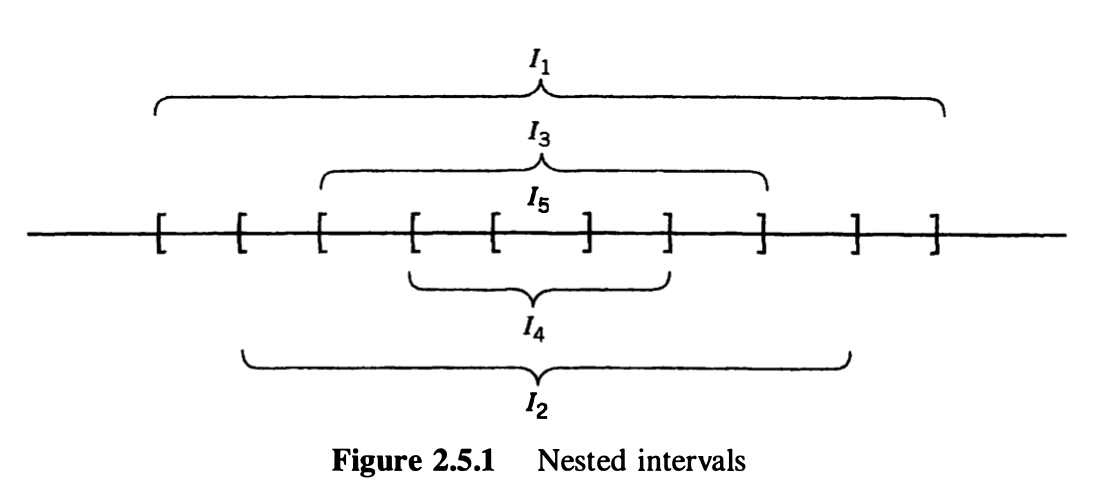
\includegraphics[width=\columnwidth]{images/nested-intervals.png}

\textbf{Theorem 2.5.1 (Nested Interval Property)} If $I_n = [a_n, b_n], n \in \mathbb{N}$ is a nested sequence of closed bounded intervals, then there exists a number $\xi \in \mathbb{R} : \xi \in I_n, \forall n \in \mathbb{N}$.

\textbf{Theorem 2.5.2} If $I_n = [a_n, b_n], n \in \mathbb{N}$ is a nested sequence of closed bounded intervals such that the lengths $b_n - a_n$ of $I_n$ satisfy

$$
\inf \{ b_n - a_n : n \in \mathbb{N} \} = 0,
$$

then the number $\xi$ contained in all $I_n$ is unique.

\subsection{Sequences and their limits}
% \textbf{Definition 3.1.1.} A \textbf{sequence} in $\mathbb{R}$ is a real-valued function $X$ with domain $\mathbb{N}$, that is

% $$
% X : \mathbb{N} \mapsto \mathbb{R}
% $$

% The numbers $X(n)$ for $n = 1, 2, 3 \cdots$ are called the \textbf{terms} of the sequence.

% \textbf{Notation} We usually write $x_n$ for $X(n)$ and denote the sequence $X$ either by $(x_n), (x_n : n \in \mathbb{N})$. Note that $(x_n : n \in \mathbb{N})$ is different from $\{ x_n : n \in \mathbb{N} \}$. Order is important for the former but not for the latter.

\textbf{Definition 3.1.3 (Definition of Limits)} $\forall \epsilon > 0, \exists K(\epsilon) \in \mathbb{N}: |x_n - x| < \epsilon, \forall n \geq K(\epsilon)$.

% \textbf{Definition 3.1.3.} A sequence $X = (x_n) \in \mathbb{R}$ is said to be \textbf{convergent} to $x \in \mathbb{R}$, or $x$ is said to be a \textbf{limit} of $(x_n)$ if for every $\epsilon > 0$, there exists a natural number $K := K(\epsilon): \forall n \geq K(\epsilon),$  the terms $x_n$ satisfy $|x_n - x| < \epsilon$. 

% If a sequence has a limit, we say that the sequence if \textbf{convergent}. Other wise, we say that the sequence is \textbf{divergent}.

% \textbf{Note:} The notation $K(\epsilon)$ is used to emphasize that the choice of $K$ depends on the value of $\epsilon$.

% \textbf{Notation} When a sequence has a limit $x$, we will use the notation

% $$
% \lim X = x \quad or \quad \lim(x_n) = x \quad or \quad \lim \underset{n \mapsto \infty}{x_n} = x
% $$

% \textbf{Theorem 3.1.1.} If $(x_n)$ converges, then it has only one limit.

% \textbf{Theorem 3.1.5} Let $X = (x_n)$ be a sequence of real numbers, and let $x \in \mathbb{R}$. The following statements are equivalent.

% (a) $X$ converges to $x$.

% (b) For every $\epsilon > 0$, there exists a natural number $K(\epsilon)$ such that for all $n \geq K(\epsilon)$, the terms $x_n$ satisfy $|x_n - x| < \epsilon$.

% (c) For every $\epsilon > 0$, there exists a natural number $K(\epsilon)$ such that for all $n \geq K(\epsilon)$, the terms $x_n$ satisfy $x - \epsilon < x_n < x + \epsilon$.

% (d) For every $\epsilon-$neighborhood $V_{\epsilon}(x)$ of $x$, there exists a natural number $K$ such that for all $n \geq K$, the terms $x_n$ belongs to $V_{\epsilon}(x)$.

% \textbf{Facts:} Let $X = (x_n)$ be a sequence of real numbers, and let $x \in \mathbb{R}$. The following statements are equivalent.

% (a) $\underset{n \mapsto \infty}{\lim} x_n = x$

% (b) $\underset{n \mapsto \infty}{\lim} x_n - x = 0$

% (c) $\underset{n \mapsto \infty}{\lim} |x_n - x| = 0$

\textbf{Theorem 3.1.9.} Let $X = (x_n : n \in \mathbb{N})$ be a sequence of real numbers and let $m \in \mathbb{N}$. Then the m-tail $X_m = (x_{m+n} : n \in \mathbb{N})$ of $X$ converges iff X converges. In this case, $\lim X_m = \lim X$.

% \textbf{Theorem 3.1.10} Let $(x_n)$ be a sequence of real numbers and let $x \in \mathbb{R}$. If $(a_n)$ is a sequence of positive real numbers with $\lim (a_n) = 0$ and if for some constant $C > 0$ and some $m \in \mathbb{N}$ we have

% $$
% |x_n - x| \leq C a_n, \forall n \geq m
% $$

% then it follows that $\lim (x_n) = x$

\textbf{Definition 3.2.1} A sequence $X = (x_n)$ of real numbers is said to be \textbf{bounded} if there exists a real number $M > 0: |x_n| \leq M, \forall n \in \mathbb{N}$.

\textbf{Theorem 3.2.2} A convergent sequence of real numbers is bounded. However, it is not true that bounded sequence implies convergence.

\textbf{Theorem 3.2.3.} If $\underset{n \mapsto \infty}{\lim} x_n = x, \underset{n \mapsto \infty}{\lim} y_n = y$ and $c \in \mathbb{R}$, then 

(i) $\underset{n \mapsto \infty}{\lim} (x_n + y_n) = x + y$;

(ii) $\underset{n \mapsto \infty}{\lim} (x_n - y_n) = x - y$;

(iii) $\underset{n \mapsto \infty}{\lim}(x_ny_n) = xy$;

(iv) $\underset{n \mapsto \infty}{\lim} c(x_n) = cx$;

(v) $\underset{n \mapsto \infty}{\lim} (x_n / y_n) = x / y$ provided $y_n \neq 0, \forall n \in \mathbb{N}$ and $y \neq 0$.

\textbf{Observations}

Let $k \in \mathbb{N}$. $\underset{n \mapsto \infty}{\lim} (a_n^k) = (\underset{n \mapsto \infty}{\lim} (a_n))^k$.

\textbf{T5Q2} If $x_n > 0$ and $\underset{n \mapsto \infty}{\lim} x_n = x \neq 0$, then $\underset{n \mapsto \infty}{\lim} (x_n)^r = x^r$ for $r \in \mathbb{Q}$.

% \textbf{T} $\underset{n \mapsto \infty}{\lim} \sqrt{(x_n)} = \sqrt{\underset{n \mapsto \infty}{\lim} (x_n)}$

% \textbf{Theorem 3.2.4} If $x_n \geq 0, \forall n \in \mathbb{N}$ and $(x_n)$ converges, then $\underset{n \mapsto \infty}{\lim} x_n \geq 0$.

% \textbf{Theorem 3.2.5} If $(x_n), (y_n)$ are convergent and $x_n \geq y_n, \forall n \in \mathbb{N}$, then 

% $$
% \underset{n \mapsto \infty}{\lim} x_n \geq \underset{n \mapsto \infty}{\lim} y_n
% $$

% \textbf{Theorem 3.2.6} If $a, b \in \mathbb{R}$ and $a \leq x_n \leq b, \forall n \in \mathbb{N}$ and $(x_n)$ is convergent, then 

% $$
% a \leq \underset{n \mapsto \infty}{\lim} x_n \leq b
% $$

\textbf{Theorem 3.2.7} (Squeeze Theorem) If $x_n \leq y_n \leq z_n, \forall n \in \mathbb{N}$ and $\underset{n \mapsto \infty}{\lim} x_n = \underset{n \mapsto \infty}{\lim} z_n = a$, then we have 

$$
\underset{n \mapsto \infty}{\lim} y_n = a
$$

\textbf{Theorem 3.2.9} Let the sequence $X = (x_n)$ converge to $x$. If $x = \lim (x_n)$, then $|x| = \lim (|x_n|)$.

% \textbf{Theorem 3.2.10} Let $X = (x_n)$ be a sequence of real numbers that converges to $x$ and suppose that $x_n \geq 0$. Then the sequence $(\sqrt{x_n})$ of positive square roots converges and $\lim (\sqrt{x_n}) = \sqrt{x}$.

\textbf{HW2Q1(c)} Let $(x_n)$ be a sequence of positive real numbers such that $L:= \lim (x_{n+1} / x_n)$ exists. If $|L| < 1$, then $(x_n)$ converges and $\lim(x_n) = 0$.

% \textbf{Definition 3.3.1} We say that the sequence $(x_n)$ is \textbf{increasing} if 

% $$
% x_1 \leq x_2 \leq \cdots x_n \leq x_{n+1} \leq \cdots
% $$

% We say that the sequence $(x_n)$ is \textbf{decreasing} if 

% $$
% x_1 \geq x_2 \geq \cdots x_n \geq x_{n+1} \geq \cdots
% $$

% We say that the sequence $(x_n)$ is \textbf{monotone} if it is either increasing or decreasing.

\textbf{Theorem 3.3.2 (Monotone Convergence Theorem)} Let $(x_n)$ be a \textbf{monotone} sequence of real numbers. Then 

$$
(x_n) \text{ is convergent } \iff (x_n)  \text{ is bounded.}
$$

Moreover,

(a) If $(x_n)$ is bounded and increasing, then $\lim x_n = \sup \{ x_n: n \in \mathbb{N} \}$

(b) If $(x_n)$ is bounded and decreasing, then $\lim x_n = \inf \{ x_n: n \in \mathbb{N} \}$

% \textbf{Definition 3.4.1}  Let $X = (x_n)$ be a sequence of real numbers and let $n_1 < n_2 < \cdots < n_k < \cdots$ be a strictly increasing sequence of natural numbers. Then the sequence $X' = (x_{n_k})$ given by 

% $$
% (x_{n_1}, x_{n_2}, \cdots, x_{n_k}, \cdots)
% $$

% is called the \textbf{subsequence} of $X$.

\textbf{Theorem 3.4.2} If $(x_n)$ converges to $x$, then any subsequence $(x_{n_k})$ also converges to $x$. That is,

$$
\underset{n_k \mapsto \infty}{\lim} x_{n_k} = \underset{k \mapsto \infty}{\lim} x_{n_k} = x.
$$

\textbf{Theorem.} If every subsequence of $(x_n)$ converges to the same limit, then the limit of $(x_n)$ is the same.

% \textbf{Theorem 3.4.4} Let $X = (x_n)$ be a sequence of real numbers. Then the following are equivalent:

% (i) The sequence $X = (x_n)$ does not converge to $x \in \mathbb{R}$.

% (ii) There exists an $\epsilon_0 > 0$ such that for any $k \in \mathbb{N}$, there exists $n_k \in \mathbb{N}$ such that $n_k \geq k$ and $|x_{n_k} - x| \geq \epsilon_0$.

% (iii) There exists an $\epsilon_0 > 0$ and a subsequence $X' = (x_{n_k})$ of $X$ such that $|x_{n_k} - x| \geq \epsilon_0$ for all $k \in \mathbb{N}$.

\textbf{Theorem 3.4.5} If a sequence $(x_n)$ has either of the following properties, then $(x_n)$ is divergent.

1. $(x_n)$ has two convergent subsequences whose limits are not equal.

2. $(x_n)$ is unbounded.

% \textbf{Theorem 3.4.7} Every sequence has a monotone subsequence.

\textbf{Theorem 3.4.8 (Bolzano-Weierstrass Theorem)} Every bounded sequence has a convergent subsequence.

% \textbf{Definition 3.5.1} A sequence $(x_n)$ is said to be a \textbf{Cauchy sequence} if $\forall \epsilon > 0, \exists H := H(\epsilon) \in \mathbb{N} > 0: |x_n - x_m| < \epsilon, \forall n, m > H$. For the negation of 3.5.1, note that there can be a relation between $n, m$.

\textbf{Definition 3.5.1 (Cauchy Sequence)} $\forall \epsilon > 0, \exists H(\epsilon) \in \mathbb{N} : |x_n - x_m| < \epsilon, \forall n, m \geq H(\epsilon)$. For the negation of 3.5.1, note that there can be a relation between $n, m$.

% \textbf{Lemma 3.5.4} A Cauchy sequence of real numbers is bounded.

\textbf{Theorem 3.5.5 (Cauchy Convergence Criterion)} A sequence of real numbers is convergent iff it is a Cauchy sequence.

\textbf{Definition 3.5.7} A sequence $(x_n)$ is called \textbf{contractive} if there exists a constant $C$, $0 < C < 1$ such that

$$
|x_{n+2} - x_{n+1}| \leq C |x_{n+1} - x_n|
$$

$\forall n \in \mathbb{N}$. The number $C$ is called the \textbf{constant} of the contractive sequence.

\textbf{Theorem 3.5.8} Every contractive sequence is Cauchy and so is convergent.

% \textbf{Definition 3.6.1} Let $(x_n)$ be a sequence of real numbers.

% (i) We say that $(x_n)$ \textbf{tends to} $+\infty$  and write $\underset{n \mapsto \infty}{\lim} x_n = + \infty$, if for every $\alpha \in \mathbb{R}$, there exists a natural number $K(\alpha)$ such that if $n \geq K(\alpha)$, then $x_n > \alpha$.

% (ii) We say that $(x_n)$ \textbf{tends to} $-\infty$  and write $\underset{n \mapsto \infty}{\lim} x_n = - \infty$, if for every $\beta \in \mathbb{R}$, there exists a natural number $K(\beta)$ such that if $n \geq K(\beta)$, then $x_n < \beta$.

% We say that $(x_n)$ is properly divergent in case we have either $\underset{n \mapsto \infty}{\lim} x_n = +\infty$ or $\underset{n \mapsto \infty}{\lim} x_n = -\infty$.

% \textbf{Remark} (i) $\pm \infty$ is \textbf{not} a real number; it's only a convenient notation. (ii) Sequences which tend to $\pm \infty$ are \textbf{divergent}.

% \textbf{Theorem 3.6.2} Let $(x_n)$ and $(y_n)$ be two sequences of real numbers and suppose that 

% $$
% x_n \leq y_n, \forall n \in \mathbb{N}
% $$

% (a) If $\underset{n \mapsto \infty}{\lim} x_n = \pm \infty$, then $\underset{n \mapsto \infty}{\lim} y_n = \pm \infty$.

% \textbf{Theorem 3.6.3(a)} If $(x_n)$ is an unbounded increasing sequence, then $\underset{n \mapsto \infty}{\lim} x_n = +\infty$.

% (b) If $(x_n)$ is an unbounded decreasing sequence, then $\underset{n \mapsto \infty}{\lim} x_n = - \infty$.

% \textbf{Summary} How to prove convergence and calculate limits: (i) Definition, (ii) Limit Theorems, (iii) Squeeze Theorem, (iv) Monotone Convergence Theorem, (v) Cauchy Criterion, contractive sequence (vi) Take the limit in the equality using m-tail sequence theorem.

\subsection{Examples for Sequences and their limits.}

\textbf{Example 3.1.6(a)} $\lim(\frac{1}{n}) = 0$.

\textbf{Example 3.1.6(b)} $\lim(\frac{1}{n^2 + 1}) = 0$.

\textbf{Example 3.1.6(d)} $\lim (\sqrt{n+1} - \sqrt{n}) = 0$.

\textbf{Example 3.1.6(e)} If $0 < b < 1$, then $\lim (b^n) = 0$.

\textbf{Example 3.1.11(c)} $c > 0 \implies \lim (c^{1 / n}) = 1$.

\textbf{Example 3.1.11(d)} $\lim (n^{1 / n}) = 1$.

\textbf{Example 3.2.8 (f)} $\lim(\frac{\sin n}{n}) = 0$.

\textbf{18/19 Midterm Q3(ii)} $\lim (\frac{\sqrt{n^3}}{\sqrt{n^3 + n}}) = 1$.

\subsection{Introduction to Infinite Series}

% \textbf{Definition 3.7.1} If $X := (x_n) $ is a sequence in $\mathbb{R}$, then the \textbf{infinite series} (or series) \textbf{generated by X} is the sequence $S := (s_k)$ defined by 

% $$
% \begin{aligned}
% s_{1} &:=x_{1} \\
% s_{2} &:=s_{1}+x_{2} \quad\left(=x_{1}+x_{2}\right) \\
% & \cdots \\
% s_{k} &:=s_{k-1}+x_{k} \quad\left(=x_{1}+x_{2}+\cdots+x_{k}\right)
% \end{aligned}
% $$

% The numbers $x_n$ are called the \textbf{terms} of the series and the numbers $s_k$ are called the \textbf{partial sums} of this series. If $\lim S$ exists, this series is \textbf{convergent} and call this limit the \textbf{sum} of the series. Else, the series $S$ is divergent.

% $$
% \sum\left(x_{n}\right) \text { or } \sum x_{n} \text { or } \sum_{n=1}^{\infty} x_{n}
% $$

% These symbols denote both the infinite series $S$ generated by the sequence $X = (x_n)$ and to denote the value $\lim S$ if the limit exists.

\textbf{Theorem 3.7.3 (the n-th term test)} If the series $\sum x_n$ converges, then $\underset{n \mapsto \infty}{\lim} x_n = 0$. Or contrapositively, if $\underset{n \mapsto \infty}{\lim} x_n$ does not exist or exists but not 0, then the series diverges.

\textbf{Theorem 3.7.4 (Cauchy criterion test)} The series $\sum x_n$ converges if and only if for every $\epsilon > 0$, there exists $M(\epsilon) \in \mathbb{N}$ such that if $m > n \geq M(\epsilon)$, then 

$$
|s_m - s_n| = |x_{n+1} + \cdots + x_m| < \epsilon
$$

\textbf{Theorem 3.7.5 (Partial sum bounded test for series with nonnegative terms} Suppose $x_n \geq 0, \forall n \in \mathbb{N}$. Then the series $\sum x_n$ converges iff the sequence $(s_n)$ of partial sums is bounded. In this case,

$$
\sum x_n = \underset{n \mapsto \infty}{\lim} s_n = \sup\{ s_n : n \in \mathbb{N} \}
$$

\textbf{Theorem 3.7.7 (Comparison Test)} Let $(x_n), (y_n)$ be real sequences and suppose that \textit{for some} $K \in \mathbb{N}$, we have

$$
\mathbf{0 \mathbf{\leq}} x_n \mathbf{\leq} y_n, \forall n \geq K
$$

Then 

(a) The convergence of $\sum y_n$ implies the convergence of $\sum x_n$.

(b) The divergence of $\sum x_n$ implies the divergence of $\sum y_n$ (contrapositive of (a)).

\textbf{Theorem 3.7.8 (Limit comparison Test)} Suppose that $(x_n), (y_n)$ are \textbf{strictly positive} sequences and suppose that the following limits exists:

$$
r := \underset{n \mapsto \infty}{\lim} (\frac{x_n}{y_n})
$$

(a) If $r > 0$ then $\sum x_n$ is convergent iff $\sum y_n$ is convergent.

(b) If $r = 0$ and if $\sum y_n$ is convergent, then $\sum x_n$ is convergent.

\textbf{Remark} 

(i) The comparison tests 3.7.7 and 3.7.8 depend on having a stock of series that one knows to be convergent (or divergent). The reader will find that the \textit{p}-series is often useful for this purpose.

(ii) Contrapositive argument for divergence test.

% \textbf{Summary} How do we test if \textit{infinite series} $(s_n)$ converge?

% (i) the $n$-th term test, (ii) Cauchy criterion test, (iii) Partial sum bounded test for series with non negative terms, (iv) comparison test, (v) limit comparison test.

\subsection{Examples for Infinite Series}

\textbf{Example 3.7.6(b)} The \textbf{harmonic series} $\sum^{\infty}_{n=1} \frac{1}{n}$ diverges.

\textbf{Example 3.7.6(c)} The \textbf{2-series} $\sum^{\infty}_{n=1} \frac{1}{n^2}$ converges.

\textbf{Example 3.7.6(d)} The \textbf{p-series} $\sum^{\infty}_{n=1} \frac{1}{n^p}$ converges when $p > 1$.

\textbf{Example 3.7.6(e)} The \textbf{p-series} $\sum^{\infty}_{n=1} \frac{1}{n^p}$ diverges when $0 < p \leq 1$.

\textbf{Example 3.7.6(f)} The alternating harmonic series given by 

$$
\sum_{n=1}^{\infty} \frac{(-1)^{n+1}}{n}=\frac{1}{1}-\frac{1}{2}+\frac{1}{3}-\cdots+\frac{(-1)^{n+1}}{n}+\cdots
$$

is convergent to $\ln 2$.

\textbf{T7Q2(b)} $\sum^{\infty}_{n=0} \frac{1}{n!} = \underset{n \mapsto \infty}{e_n} = e$. The series converges.

\textbf{T7Q2(c)} $\sum^{\infty}_{n=0} (1 + \frac{1}{n})^n$ converges.

\section{Infinite Series}

\subsection{Absolute Convergence}

\textbf{Definition 9.1.1} The series $\sum x_n$ is \textbf{absolutely convergent} if the series $\sum |x_n|$ is convergent. A series is said to be \textbf{conditionally (or nonabsolutely) convergent} if it is convergent, but it is \textbf{not} absolutely convergent.

\textbf{Theorem 9.1.2} If a series $\sum^{\infty}_{n=1} x_n$  is absolutely convergent, then it is convergent.

\subsection{Tests for Absolute Convergence}

\textbf{Theorem 9.2.1 (Limit Comparison Test II)} Suppose that $(x_n), (y_n)$ are non-zero sequences and suppose that the following limits exists:

$$
r := \underset{n \mapsto \infty}{\lim} (\frac{|x_n|}{|y_n|})
$$

(a) If $r > 0$, then $\sum x_n$ is \textit{absolutely convergent} iff $\sum y_n$ is \textit{absolutely convergent}.

(b) If $r = 0$ and $\sum y_n$ is \textit{absolutely convergent}, then $\sum x_n$ is absolutely convergent.

\textbf{Theorem 9.2.2 (Root Test)} Let $(x_n)$ be a sequence

(a) If there exist $r \in \mathbb{R}$ with $0 \leq r < 1$ and $K \in \mathbb{N}$ such that 

$$
|x_n|^{\frac{1}{n}} \leq r \quad \forall n \geq K
$$

then the series $\sum x_n$ is absolutely convergent.

(b) If there exists $K \in \mathbb{N}$ such that

$$
|x_n|^{\frac{1}{n}} \geq 1 \quad \forall n \geq K
$$

then the series $\sum x_n$ is divergent.

\textbf{Corollary 9.2.3} Suppose that the limit $r := \underset{n \mapsto \infty}{\lim} |x_n|^{\frac{1}{n}}$ exists. Then $\sum x_n$ is absolutely convergent when $r < 1$ and is divergent when $r > 1$.  

\textbf{Remark.} 
(i) If $r = 1$, the root test provides no information.

(ii) Corollary 9.2.3 uses $\lim$ while Theorem 9.2.2 uses upper/lower bound.

\textbf{Theorem 9.2.4 (Ratio Test)} Let $(x_n)$ be a sequence of nonzero real numbers.

(a) If there exist $r$ with $0 < r < 1$ and $K \in \mathbb{N}$ such that

$$
|\frac{x_{n+1}}{x_n}| \leq r \quad \forall n \geq K
$$

then $\sum x_n$ is absolutely convergent.

(b) If there exists $K \in \mathbb{N}$ such that 

$$
|\frac{x_{n+1}}{x_n}| \geq 1 \quad \forall n \geq K
$$

then $\sum x_n$ is divergent.

\textbf{Corollary 9.2.5} Let $(x_n)$ be a sequence of nonzero real numbers and suppose that the limit $r := \underset{n \mapsto \infty}{\lim} |\frac{x_{n+1}}{x_n}|$ exists. Then $\sum x_n$ is absolutely convergent when $r < 1$ and is divergent when $r > 1$.

\section{Limits}

\subsection{Limits of Functions}

\textbf{Definition 4.1.1} Let $A$ be a subset of $\mathbb{R}$. A point $c$ is called a \textbf{cluster point} of $A$ if for every $\delta > 0$, there exists at least one point $x \in A, x \neq c$ such that $|x - c| < \delta$ or $c - \delta < x < c + \delta$. Alternatively,

$$
(V_{\delta}(c) \backslash \{ c \}) \cap A \neq \emptyset \text{ for any } \delta > 0
$$

\textbf{Definition 4.1.4} Let $A \subseteq \mathbb{R}$ and $c$ be a cluster point of $A$. For a function $f: A \mapsto \mathbb{R}$, a real number $L$ is said to be a \textbf{limit} of $f$ at $c$ if for any given $\epsilon > 0$, there exists a $\delta = \delta(\epsilon) > 0$ such that if $x \in A$ and $0 < |x - c| < \delta$, then $|f(x) - L| < \epsilon$, that is,

$$
x \in A \cap (V_{\delta}(c) \backslash \{ c \}) \implies f(x) \in V_{\epsilon}(L)
$$

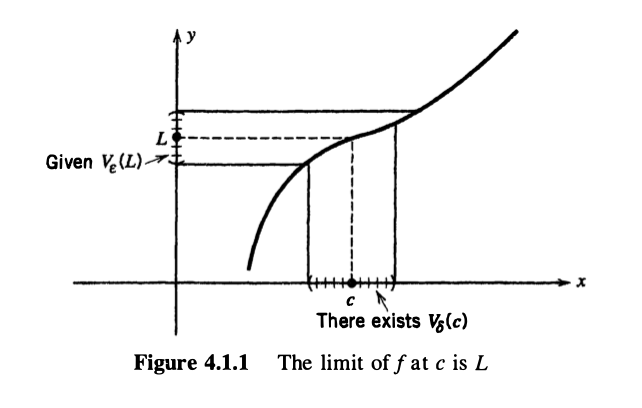
\includegraphics[width=\columnwidth]{images/function-limits-definition.png}

\textbf{Remark}

1. The cluster point $c$ does not necessarily belong to $A$. Thus to discuss the limit of $f$ at a point $x = c$, we do not require $f$ to be defined at $x = c$.

2. Even if $f(c)$ is defined, its value has no bearing on $\underset{x \mapsto c}{\lim} f(x)$.

\textbf{Definition} If $f$ has no limit at $x = c$, then we say that $f$ diverges at $c$.

% \textbf{Theorem 4.1.2} A real number $c$ is a cluster point of $A$ iff there exists a sequence $(a_n)$ in $A$ such that $\lim a_n = c$ and $a_n \neq c,  \forall n \in \mathbb{N}$.

% \textbf{Strategy: $\underset{x \mapsto c}{\lim} f(x) = L$}.

% \textit{Goal:} Find positive $\delta$ (depending on $\epsilon$) such that if $0 < |x - c| < \delta$, then $|f(x) - L| < \epsilon$.

% 1. Study $|f(x) - L|$ and try to factorize as $\frac{|f(x) - L|}{|x - c|} \times |x - c|$.

% 2. Assume that we can find a bound $M$ of $\frac{|f(x) - L|}{|x - c|}$ for $x \in V_1(c)$, i.e.

% $$
% \frac{|f(x) - L|}{|x - c|} \leq M,
% $$

% \textbf{where 1 is just a test choice} in order to obtain a bound $M$.

% 3. Then $|f(x) - L| = \frac{|f(x) - L|}{|x - c|} \times |x - c| \leq M|x - c|$.

% 4. We may take $\delta = \min \{ \frac{\epsilon}{M}, \mathbf{1} \}$ and obtain for any $x \in V_{\delta}(c)$,

% $$
% |f(x) - L| \leq M|x - c| < M \cdot \frac{\epsilon}{M}= \epsilon
% $$

% \textbf{Remark.}

% You may replace 1 by any concrete number for obtaining a convenient bound M.

% Sometimes, it might be difficult to obtain equation in 2. directly. But the main goal is still to obtain equation in 4.

% \textbf{Theorem 4.1.5} If $f: A \mapsto \mathbb{R}$ and if $c$ is a cluster point of $A$, then $f$ can have only one limit at $c$.

\textbf{Theorem 4.1.8 (Sequential Criterion for Limits of Functions)} Let $f : A \mapsto \mathbb{R}$ and $a$ be a cluster point of $A$. The following statements are equivalent:

1. $\underset{x \mapsto a}{\lim} f(x) = L$

2. For every sequence $(x_n)$ in $A$ that converges to $a$ such that $x_n \neq a$ for all $n$, the sequence $(f(x_n))$ converges to $L$.

% 2. $x_n \mapsto c$ and $x_n \in A, x_n \neq c, \forall n \in \mathbb{N}$, then $f(x_n) \mapsto L$.

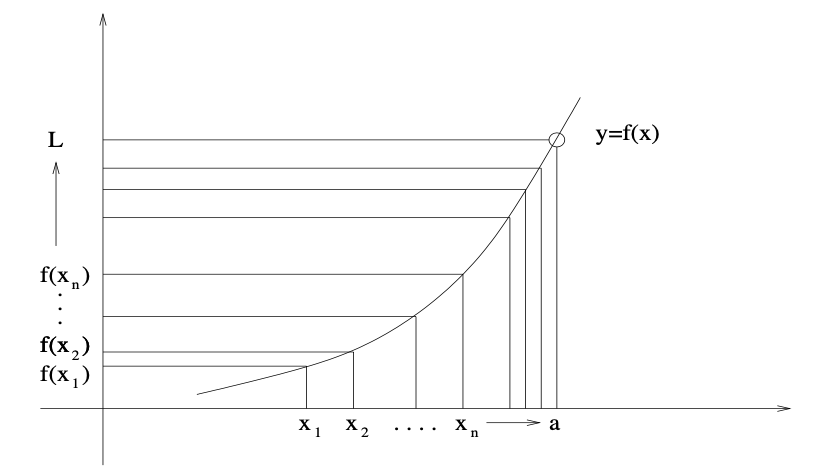
\includegraphics[width=\columnwidth]{images/sequential-criterion-limit.png}

\subsection{Limit Theorems}

\textbf{Definition 4.2.1} Let $f : A \mapsto \mathbb{R}$ and $c$ be a cluster point of $A$. We say that $f$ is \textbf{bounded on a neighbourhood of $c$} if there exists $V_{\delta}(c)$ and a constant $M > 0$ such that $|f(x)| \leq M$ for all $x \in A \cap V_{\delta}(c)$.

\textbf{Theorem 4.2.2} If $f : A \mapsto \mathbb{R}$ has a limit at a cluster point $c$, then $f$ is bounded on some neighbourhood of $c$.

\textbf{Definition 4.2.3} Let $A \subset \mathbb{R}$ and let $f$ and $g$ be functions defined on $A$. We define the \textbf{sum} $f + g$, the \textbf{difference} $f - g$, and the \textbf{product} $fg$ on $A$ to be the functions given by 

$$
\begin{aligned}
& (f+g)(x) := f(x) + g(x) \\
& (f-g)(x) := f(x) - g(x) \\
& (fg)(x) := f(x)g(x)
\end{aligned}
$$

If $b \in \mathbb{R}$, we define the \textbf{multiple} $bf$ to be the function given by 

$$
(bf)(x) := bf(x)
$$

If $h(x) \neq 0, \forall x \in A$, we define the \textbf{quotient} $f / h$ to be the function given by 

$$
(\frac{f}{h})(x) := \frac{f(x)}{h(x)}
$$

\textbf{Theorem 4.2.4} Suppose that $\underset{x \mapsto c}{\lim} f(x) = L$ and $\underset{x \mapsto c}{g(x)} = M$. Let $b \in \mathbb{R}$.

(a) $\underset{x \mapsto c}{\lim} (f \pm g)(x) = L \pm M$;

(b) $\underset{x \mapsto c}{\lim} (fg)(x) = LM, \underset{x \mapsto c}{\lim} (bf)(x) = bL$;

(c) If $h(x) \neq 0, \forall x \in A$ and $\underset{x \mapsto c}{\lim} h (x) = H \neq 0$, then 

$$
\underset{x \mapsto c}{\lim} (\frac{f}{h}) (x) = \frac{L}{H}.
$$

\textbf{Remark} Let $f_1, \cdots, f_n$ be functions on $A$ to $\mathbb{R}$. Assume that $\underset{x \mapsto c}{\lim} f_i(x) = L_i, 1 \leq i \leq n$.

1. $\underset{x \mapsto c}{\lim} (f_1 + \cdots + f_n) (x) = L_1 + \cdots + L_n$.

2. $\underset{x \mapsto c}{\lim} (f_1 \cdot \cdots \cdot f_n) (x) = L_1 \cdot \cdots \cdot L_n$.

3. If $L = \underset{x \mapsto c}{\lim} f$ and $n \in \mathbb{N}$, then $\underset{x \mapsto c}{\lim} (f(x)^n) = (\underset{x \mapsto c}{\lim} f(x))^n = L^n$.

% \textbf{Theorem 4.2.6} If $f(x) \leq g(x)$ for all $x \in A$ and both $\underset{x \mapsto c}{\lim} f(x)$ and $\underset{x \mapsto c}{\lim} g(x)$ exist, then 

% $$
% \underset{x \mapsto c}{\lim} f(x) \leq \underset{x \mapsto c}{\lim} g(x)
% $$

\textbf{Theorem 4.2.7 (Squeeze Theorem)} Let $A \subseteq \mathbb{R}$, let $f, g, h : A \mapsto \mathbb{R}$ and let $c \in \mathbb{R}$ be a cluster point of $A$. Suppose that $f(x) \leq g(x) \leq h(x)$ for all $x \in A$ and $\underset{x \mapsto c}{\lim} f(x) = \underset{x \mapsto c}{\lim} h(x) = L$, then 

$$
\underset{x \mapsto c}{\lim} g(x) = L.
$$

\textbf{Theorem 4.2.9 (Lower Bound)} If $\underset{x \mapsto c}{\lim} f(x) > 0$ (resp. $\underset{x \mapsto c}{\lim} f(x) < 0$), then there exists $V_{\delta}(c)$ of $c$ such that  $f(x) > 0$ (resp. $f(x) < 0$) for all $x \in A \cap V_{\delta}(c), x \neq c$.

\textbf{Remark.} Lower bound theorem can be applied to continuous points as well since $\underset{n \mapsto \infty}{\lim} f(x) = f(c)$ iff $f$ is continuous at $c$.

\textbf{Definition 4.3.1 (One-sided limit)} Let $f$ be a function on $A$ to $\mathbb{R}$.

(i) Let $c$ be a cluster point of $A \cap (c, \infty).$ We say that $L$ is the \textbf{right-hand limit} of $f$ at $c$ if for any $\epsilon > 0$, $\exists \delta > 0:$

$$
\mathbf{0 < x - c < \delta} (i.e. x \in (c, c + \delta)) \implies |f(x) - L| < \epsilon
$$

In this case, we write $\underset{x \mapsto c^+}{\lim} f(x) = L$.

(ii) Let $c$ be a cluster point of $A \cap (-\infty, c)$. We say that $L$ is the \textbf{left-hand limit} of $f$ at $c$ if for any $\epsilon > 0$, $\exists \delta > 0:$

$$
\mathbf{-\delta < x - c < 0}  (i.e. x \in (c - \delta, c)) \implies |f(x) - L| < \epsilon
$$

In this case, we write $\underset{x \mapsto c^-}{\lim} f(x) = L$.

\textbf{Theorem 4.3.2 (Sequential Criterion for one-sided limits)}.

(i) $\underset{x \mapsto c^+}{\lim} f(x) = L \iff $ if for every $(x_n)$ converges to $c$ and $x_n > c$ for all $n \in \mathbb{N}$, the sequence $(f(x_n))$ converges to $L$.

(ii) $\underset{x \mapsto c^-}{\lim} f(x) = L \iff$ for every $(x_n)$ converges to $c$ and $x_n < c$ for all $n \in \mathbb{N}$, the sequence $(f(x_n))$ converges to $L$.

\textbf{Theorem 4.3.3} $\underset{x \mapsto c}{\lim} f(x) = L$ exists iff both $\underset{x \mapsto c^+}{\lim} f(x)$ and $\underset{x \mapsto c^-}{\lim} f(x)$ exist and

$$
\underset{x \mapsto c^+}{\lim} f(x) = \underset{x \mapsto c^-}{\lim} f(x) = L.
$$

\section{Continuous Functions}

\subsection{Continuous Functions}

\textbf{Definition 5.1.1 ($\epsilon-\delta$ definition of continuity)} Let $A \subset R$, let $f : A \mapsto \mathbb{R}$ and let $c \in A$. We say that $f$ is \textbf{continuous at c} if given any number $\epsilon > 0$, there exists $\delta > 0$ such that if $x$ is any point of $A$ satisfying $|x - c| < \delta$, then $|f(x) - f(c)| < \epsilon$.

\textbf{Equivalent Definition to 5.1.1.}  If $c$ is a cluster point in $A$, $f(x)$ is continuous at $c$ iff

$$
f(c) = \underset{x \mapsto c}{\lim} f(x)
$$

\textbf{Remark.} The equivalent definition is useful as it opens up limit theorems (e.g. squeeze theorem, lower bound etc).

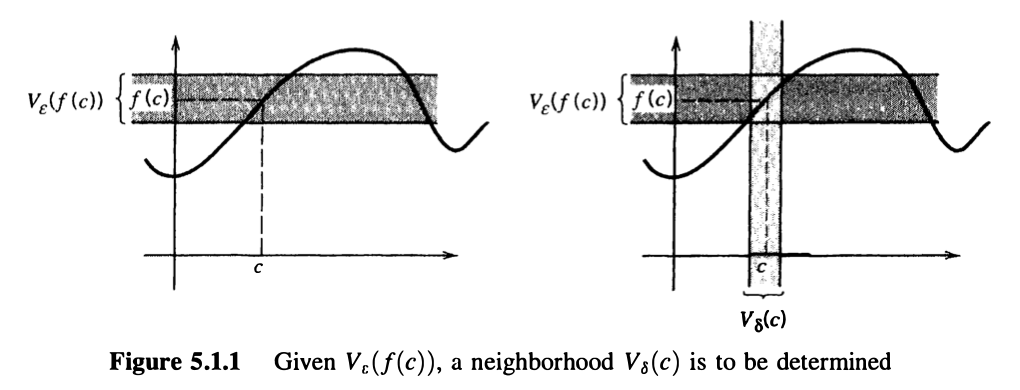
\includegraphics[width=\columnwidth]{images/continuous-function-definition.png}

\textbf{Remarks}

(i) Limit has to exist (i.e. left and right limit must exist and be the same.)

(ii) Equality must hold

(iii) $f(c)$ must be well defined.

% \textbf{Theorem 5.1.2} Let $A \subset R$, let $f : A \mapsto \mathbb{R}$ and let $c \in A$. We say that $f$ is \textbf{continuous at c} if given any $\epsilon-$neighbourhood $V_{\epsilon}(f(c))$ of $f(c)$, there exists a $\delta-$neighbourhood $V_{\delta}(c)$ of $c$ such that if $x$ is any point of $A \cap V_{\delta}(c)$, then $f(x)$ belongs to $V_{\epsilon}(f(c))$, that is

% $$
% f(A \cap V_{\delta} (c)) \subseteq V_{\epsilon}(f(c))
% $$

% (i) If $f$ fails to be continuous at $c$, then we say that $f$ is \textbf{discontinuous} at $c$.

% (ii) If $f$ is continuous at every point in $A$, then we say that $f$ is \textbf{continuous on $A$}.

% (iii) In the definition $f(c) = \underset{x \mapsto c}{\lim} f(x)$, $c$ is a cluster point and $c \in A$ (i.e. $f$ must be defined at $c$). The limit of $f(x)$ exists as $x \mapsto c$.

% (iv) If $c \in A$ is not a cluster point, then $\exists \delta > 0: V_{\delta}(c) \cap A = \{ c \}$. Such point $c$ is called an `isolated' point in $A$. By definition, $f$ is automatically continuous at $c$. But such continuity is of less interest.

\textbf{Theorem 5.1.3} (Sequential Criterion for Continuity) A function $f : A \mapsto \mathbb{R}$ is continuous at the point $c \in A$ iff for every sequence $(x_n)$ in $A$ that converges to $c$, the sequence $(f(x_n))$ converges to $f(c)$.

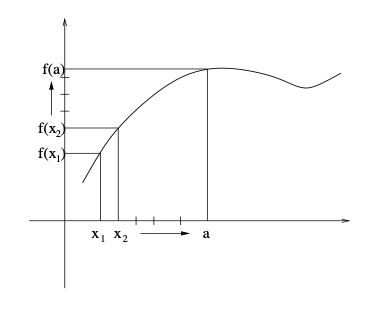
\includegraphics[width=\columnwidth]{images/sequential-criterion-continuity.png}

\textbf{Theorem 5.1.4} (Discontinuity Criterion) $f$ is discontinuous at $x = a$ iff there \textbf{exists} a sequence $(x_n)$ in the domain of $f$ such that $x_n \mapsto a$, but $f(x_n) \nrightarrow f(a)$. 

\textbf{Remark} (i) $(f(x_n))$ is divergent or (ii) $\underset{n \mapsto \infty}{\lim} f(x_n) \neq f(a)$.

\subsection{Combinations of Continuous Functions}

\textbf{Theorem 5.2.1} Suppose that $f$ and $g$ are continuous at $x = c$, then

(a) $f \pm g, f \cdot g,$ and $bf$ are also continuous at $x = c$, where $b$ is a constant.

(b) If $g(c) \neq 0$, then $f / g$ is also continuous at $x = c$.

\textbf{Theorem 5.2.2} Suppose that $f$ and $g$ are continuous on $A$, then 

(a) $f \pm g, f \cdot g, $ and $bf$ are also continuous on $A$.

(b) If $g(c) \neq 0$, then $f / g$ is also continuous on $A$.

% \textbf{Definition} If $f : A \mapsto \mathbb{R}, g : B \mapsto \mathbb{R}$ and $f(A) \subseteq B$ (i.e. $\mathcal{R}(f) \subseteq B$, then we define the \textbf{composition function} $g \circ f: A \mapsto \mathbb{R}$ by

% $$
% (g \circ f)(x) = g(f(x)), \quad \forall x \in A
% $$

% 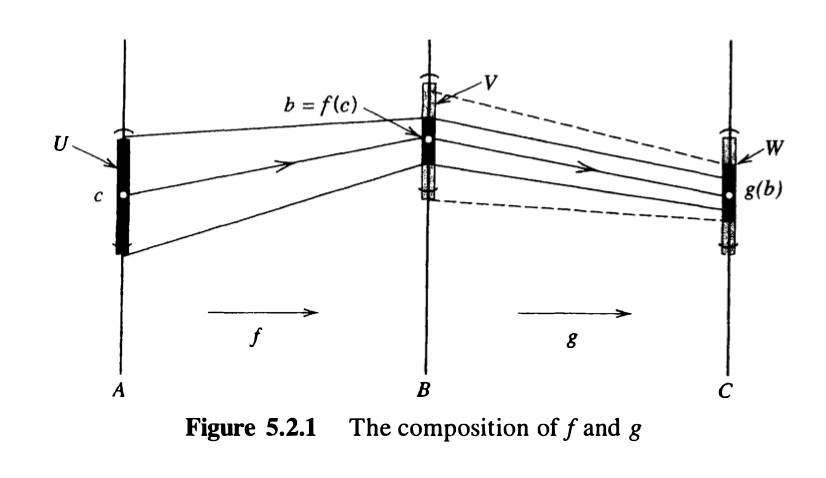
\includegraphics[width=\columnwidth]{images/function-composition.png}

\textbf{Theorem 5.2.6} Let $f : A \mapsto \mathbb{R}, g : B \mapsto \mathbb{R}$ and $f(A) \subseteq B$. If $f$ is continuous at $c$, and $g$ is continuous at $b = f(c)$, then $g \circ f$ is continuous at $c$.

\textbf{Theorem 5.2.7} Let $f : A \mapsto \mathbb{R}, g : B \mapsto \mathbb{R}$ and $f(A) \subseteq B$. If $f$ is continuous at $A$, and $g$ is continuous at $B$, then $g \circ f$ is continuous on $A$.

% \textbf{Remark.} If $f$ is defined on the closed interval $[a, b]$, then $f$ is continuous on $[a, b]$ iff

% (i) $f$ is continuous on $(a, b)$ in the usual sense, i.e. $\underset{x \mapsto c}{\lim} f(x) = f(c), \forall c \in (a, b)$.

% (ii) $\underset{x \mapsto a^+}{\lim}f(x) = f(a)$ and $\underset{x \mapsto a^-}{\lim}f(x) = f(b)$ .

% This remark just explicates definition 5.1.1 in the case $A = [a, b]$.

\subsection{Continuous Functions on Intervals}

\textbf{Definition 5.3.1} A function $f: A \mapsto \mathbb{R}$ is \textbf{bounded} on $A$ if there exists $M > 0$ such that 

$$
|f(x)| \leq M, \forall x \in A
$$

Or, the set $f(A)$ is bounded.

% \textbf{Theorem 5.3.2 (Boundedness Theorem)} If $f$ is continuous on $[a, b]$, then $f$ is bounded on $[a, b]$. 

% \textbf{Remark}

% (i) The interval must be bounded

% (ii) The interval must be closed. (i) and (ii) implies 1) the cluster points of $[a, b]$ is the set $[a, b]$ itself and 2) Let $(x_{n_k}) \subset [a, b]$ denote the convergent subsequence and let $c = \underset{k \mapsto \infty}{\lim} (x_{n_k})$. Since $a \leq x_{n_k} \leq b \enskip \forall k \in \mathbb{N}$, then $a \leq c \leq b$. Note that $a < x_{n_k} < b$ does not imply $a < c < b$.

% (iii) The function must be continuous.

\textbf{Definition 5.3.3} (i) We say that $f$ has an \textbf{absolute maximum} on $A$ if there exists $x^* \in A$ such that 

$$
f(x^*) \geq f(x), \forall x \in A.
$$

So in this case, $f(x^*) = \sup f(A) = \max f(A)$.

(ii) We say that $f$ has an \textbf{absolute minimum} on $A$ if there exists $x_* \in A$ such that 

$$
f(x_*) \leq f(x), \forall x \in A.
$$

So in this case, $f(x_*) = \inf f(A) = \min f(A)$.

\textbf{Theorem 5.3.4 (Maximum-Minimum Theorem)} If $f$ is continuous on $[a, b]$, then $f$ has an absolute maximum and an absolute minimum on $[a, b]$.

\textbf{Bisection Method.} Essentially Binary Search.

\textbf{Theorem 5.3.5 (Location of Roots Theorem)} If $f$ is continuous on $[a , b]$ and $f(a)f(b) < 0$, then there exists a point $c \in (a, b)$  such that $f(c) = 0$.

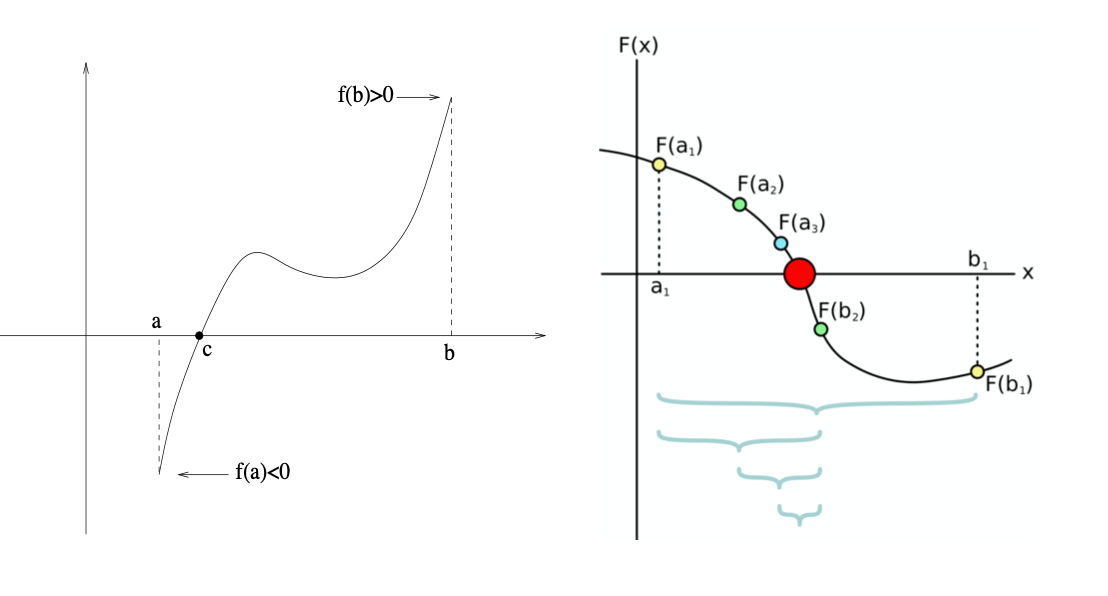
\includegraphics[width=\columnwidth]{images/location-of-roots.png}

\textbf{Theorem 5.3.7 (Intermediate Value Theorem)} Let $I$ be an interval, $f$ be continuous on $I$, and $a, b \in I$ with $f(a) \leq f(b)$. For any $k \in [f(a), f(b)]$, then there exists a point $c$ in $I$ such that $f(c) = k$. 

\textbf{Remark.} $a, b \in I$. (i) Case $a \leq b$: $[a, b] \subseteq I$ (ii) Case $b > a$: $[b, a] \subseteq I$.

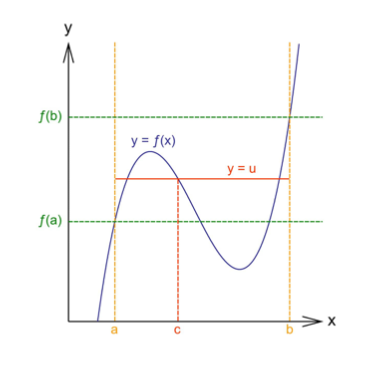
\includegraphics[width=\columnwidth]{images/intermediate-value-theorem.png}

\textbf{Theorem 5.3.10 (Preservation of Closed Intervals Theorem)} If $f$ is continuous on $[a ,b]$, then 

$$
f([a, b]) := \{ f(x) : x \in [a, b] \} = [m, M]
$$

where $m = \inf f([a, b]) = f(x_*)$ and $M = \sup f([a, b]) = f(x^*)$. That is, for any $m \leq k \leq M$, there exists $c \in [a, b]$ such that $f(c) = k$.

\textbf{Remark.} Let $f$ be a continuous function on $[a, b]$.

1. $f([a, b]) = [m, M]$ does not imply $f([a, b]) = [f(a), f(b)]$. Image of the closed interval might not equal the closed interval given by $f(a), f(b)$.

2. If we replace the closed bounded interval $[a, b]$ by an arbitrary interval $I$ (e.g. open or half-open), then $f(I)$ could be of any type such as half-open or unbounded.

\subsection{Uniform Continuity}

\textbf{Uniform Continuity} Let $A \subset \mathbb{R}$, $f: A \mapsto \mathbb{R}$. We say that $f$ is \textbf{uniformly continuous} on $A$ if for each $\epsilon > 0$, there exists a $\delta(\epsilon) > 0$ ($\delta (\epsilon)$ only depends on $\epsilon$) such that 

$$
\forall x, y \in A, |x - y| < \delta(\epsilon) \implies |f(x) - f(y)| < \epsilon
$$

\textbf{Negative Definition.} $f$ is \textbf{not uniformly continuous} on $A$ if there exists an $\epsilon_0 > 0$ such that for all $\delta > 0$, there are points $x_{\delta}, y_{\delta}$ such that $|x_{\delta} - y_{\delta}| < \delta$ and $|f(x_{\delta}) - f(y_{\delta})| \geq \epsilon_0$.

\textbf{(Sequential Criterion for Uniform Continuity)} The function $f: A \mapsto \mathbb{R}$ is uniformly continuous on $A$ iff for any two sequences $(x_n), (y_n)$ in $A$ such that $\underset{n \mapsto \infty}{\lim} x_n - y_n = 0$, we have $\underset{n \mapsto \infty}{\lim} f(x_n) - f(y_n) = 0$.

\textbf{Negative Definition.} There exists an $\epsilon_0 > 0$ and two sequences $(x_n), (y_n)$ in $A$ such that $\underset{n \mapsto \infty}{\lim} x_n - y_n = 0$ and we have $\underset{n \mapsto \infty}{\lim} |f(x_n) - f(y_n)| \geq \epsilon_0$.

\textbf{Theorem 5.4.3 (Uniform Continuity Theorem)} If $f$ is continuous on a closed bounded interval $[a, b]$, then it is uniformly continuous on $[a, b]$.

\textbf{Definition 5.4.4} A function $f: A \mapsto \mathbb{R}$ is said to be a \textbf{Lipschitz function} (or satisfy a \textbf{Lipschitz condition}) on $A$ if there exists a $K > 0$ such that 

% $$
% |f(x) - f(y)| \leq K|x - y|, \forall x, y \in A
% $$

% \textbf{Remark.} We can write the condition as 

$$
\frac{|f(x) - f(y)|}{|x - y|} \leq K, \text{ for } x \neq y \in A
$$

which implies that its \textit{derivative} $f'(x)$ (if exists) is bounded on $A$.

\textbf{Theorem 5.4.5} If $f: A \mapsto \mathbb{R}$ is a Lipschitz function, then $f$ is uniformly continuous on $A$.

\textbf{Theorem 5.4.7 (Uniformly continuous functions preserve Cauchy sequence)} If $f: A \mapsto \mathbb{R}$ is uniformly continuous on $A$ and $(x_n)$ is a Cauchy sequence in $A$, then $(f(x_n))$ is a Cauchy sequence.

\textbf{Theorem 5.4.8 (Continuous Extension Theorem)} A function $f$ is uniformly continuous on the interval $(a , b)$ iff $\underset{x \mapsto a^+}{\lim} f(x)$ and $\underset{x \mapsto b^-}{\lim} f(x)$ can be defined at the endpoints $a$ and $b$ such that the extended function is continuous on $[a, b]$.

\subsection{Monotone and Inverse Functions}

\textbf{Theorem 5.6.1 (One-sided Limits for Monotone Functions Exist Theorem)} Let $I \subset \mathbb{R}$ be an interval and let $f : I \mapsto \mathbb{R}$ be \textbf{increasing} on $I$. Suppose that $c \in I$ is not an endpoint of $I$. Then 

(i) $\underset{x \mapsto c^-}{\lim} f(x) = \sup \{ f(x): x \in I, x < c \}$

(ii) $\underset{x \mapsto c^+}{\lim} f(x) = \inf \{ f(x): x \in I, x > c \}$

\textbf{Remark.} By showing limit exists, we can also use theorems related to limits such as the sequential criterion for limits theorem.

% \textbf{Corollary 5.6.2} Let $I \in \mathbb{R}$ be an interval and let $f: I \mapsto \mathbb{R}$ be \textbf{increasing} on $I$. Suppose that $c \in I$ is not an endpoint of $I$. Then the following statements are equivalent:

% (a) $f$ is continuous at $c$

% (b) $\underset{x \mapsto c^-}{\lim} f(x) = f(c) = \underset{x \mapsto c^+}{\lim} f(x)$

% (c) $\sup \{ f(x): x \in I, x < c \} = f(c) = \inf \{ f(x): x \in I, x > c \} $

\textbf{Definition} If $f : I \mapsto \mathbb{R}$ is \textbf{increasing} on $I$ and if $c$ is not an endpoint of $I$, we define the \textbf{jump of $f$ at $c$} to be 

$$
\begin{aligned}
    &j_f(c) := \underset{x \mapsto c^+}{\lim} f(x) - \underset{x \mapsto c^-}{\lim} f(x) \\
           &= \mathbf{\inf} \{ f(x): x \in I, x > c \} - \mathbf{\sup} \{ f(x): x \in I, x < c \} 
\end{aligned}
$$

At the endpoints $a$ or $b$, define

$$
j_{f}(c):=\left\{\begin{array}{ll}
\underset{x \rightarrow a^{+}}{\lim} f(x)-f(a) & \text { if } c=a \\
f(b)-\underset{x \rightarrow b^{-}}{\lim} f(x) & \text { if } c=b
\end{array}\right.
$$

\textbf{Theorem 5.6.3} Let $f : I \mapsto \mathbb{R}$ be \textbf{increasing} on $I$. Then $f$ is continuous at $c$ iff $j_f(c) = 0$.

\textbf{Remark.} Theorem 5.6.1, Corollary 5.6.2, defn of Jump, and theorem 5.6.3 can be reformulated from \textbf{increasing} to \textbf{decreasing} functions.

\textbf{Theorem 5.6.4 (Discontinuous points of monotone functions)} Let $I \subseteq \mathbb{R}$ be an interval and let $f: I \mapsto \mathbb{R}$ be monotone on $I$. Then the set of points $D \subseteq I$ at which $f$ is discontinuous is a countable set.

% \textbf{Remark.} In other words, a monotone function can only have countably many discontinuities in its domain. Thus CDF, which is a bounded increasing function, has countably many discontinuous points.

\textbf{Theorem 5.6.5 (Continuous Inverse Theorem)} Let $I \subset \mathbb{R}$ be an interval and $f : I \mapsto \mathbb{R}$ be \textbf{strictly} monotone and continuous. Then the inverse function $f^{-1}$ is also strictly monotone and continuous on $J := f(I) = \mathcal{R}(f)$.

\textbf{Remark.} $f^{-1}: J \mapsto \mathbb{R}$, where $J$ might not equal the codomain of $f$.

\textbf{Rational Power Function.} $x^r, r \in \mathbb{Q}$ is defined.

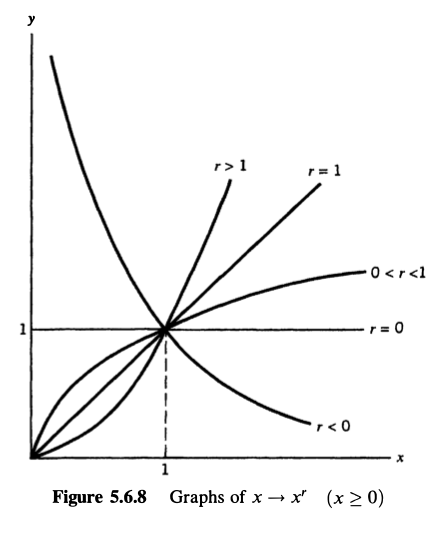
\includegraphics[width=\columnwidth]{images/rational-power.png}

\textbf{Theorem 5.6.7} If $m \in \mathbb{Z}, n \in \mathbb{N}$ and $x > 0$, then $(x^{{\frac{1}{n}})^m} = (x^m)^{\frac{1}{n}}$

\section{A Glimpse into Topology}
\subsection{Open and Closed Sets in $\mathbb{R}$}

\textbf{Definition 11.1.1} A set $V$ is called a \textbf{neighbourhood} of a point $x \in \mathbb{R}$ if $\exists \epsilon > 0: V_{\epsilon}(x) \subseteq V$.

\textbf{Definition 11.1.2} 

% (i) A subset $G$ of $\mathbb{R}$ is \textbf{open} in $\mathbb{R}$ if $\forall x \in G$, there exists a neighbourhood $V$ of $x$ such that $V \subseteq G$. Equivalently, $\forall x \in G, \exists \epsilon_x > 0: V_{\epsilon_x}(x) \subseteq G$.

(i) A subset $G$ of $\mathbb{R}$ is \textbf{open} in $\mathbb{R}$ if $G$ is a neighbourhood of any point in $G$, that is, $\forall x \in G, \exists \epsilon_x > 0: V_{\epsilon_x}(x) \subseteq G$.

(ii) A subset $F$ of $\mathbb{R}$ is \textbf{closed} in $\mathbb{R}$ if the complement $C(F) := \mathbb{R} \backslash F$ is open in $\mathbb{R}$. Equivalently, for any $y \notin F, \exists \epsilon_0 > 0: V_{\epsilon_0}(y) \cap F = \emptyset$.

\textbf{Theorem 11.1.4 (Open Set Properties)} 

(a) The union of an arbitrary collection of open subsets in $\mathbb{R}$ is open. 

(b) The intersection of any \textbf{finite} collection of open sets in $\mathbb{R}$ is open. 

\textbf{Theorem 11.1.5 (Closed Set Properties)} 

(a) The intersection of an arbitrary collection of closed subsets in $\mathbb{R}$ is closed

(b) The union of any finite collection of closed sets in $\mathbb{R}$ is closed.

\textbf{Theorem 11.1.7 (Characterisation of Closed Sets)} A subset $F$ of $\mathbb{R}$ is closed iff for any convergent sequence $(x_n)$ in $F$, $\underset{n \mapsto \infty}{\lim} x_n$ belongs to $F$.

\textbf{Theorem 11.1.8} A subset $F$ of $\mathbb{R}$ is closed iff it contains all of its cluster points.

\textbf{Theorem 11.1.9 (Characterisation of Open Sets)} A subset of $\mathbb{R}$ is open iff it is the union of countably many disjoint open intervals in $\mathbb{R}$.

\subsection{Continuous Functions}
\textbf{Lemma 11.3.1} A function $f: A \mapsto \mathbb{R}$ is continuous at the point $c$ in $A$ iff for every (open) neighborhood $U$ of $f(c)$, there exists a (open) neighborhood $V$ of $c$ such that if $x \in V \cap A$, then $f(x) \in U$. That is, $\forall$ neighborhood $U$ of $f(c)$, $\exists$ a neighborhood $V$ of c st. $f(V \cap A) \subseteq U$.

\textbf{Theorem 11.3.2 (Global Continuity Theorem)} Let $f: A \mapsto \mathbb{R}$ be a function with domain $A$. Then the following are equivalent:

(a) $f$ is continuous at every point of $A$.

(b) For every open set $G$ in $\mathbb{R}$, there exists an open set $H$ in $\mathbb{R}$ such that $H \cap A = f^{-1}(G)$.

Note that for a set $G$, $f^{-1}(G) := \{ x \in A: f(x) \in G\}$ (preimage, not inverse!). 

\textbf{Corollary 11.3.3} A function $f: \mathbb{R} \mapsto \mathbb{R}$ is continuous iff $f^{-1}(G)$ is open in $\mathbb{R}$, whenever $G$ is open. Or, the preimage of an open set is always open.

\textbf{Remark.} In general, for an open set $G$, the direct image $f(G)$ is not necessarily open.

\subsection{Metric Spaces}

\textbf{Definition 11.4.1} A \textbf{metric} on a set $S$ is a function $d: S \times S \mapsto \mathbb{R}$ that satisfies the following properties:

(a) $d(x ,y) \geq 0, \forall x, y \in S$ (positivity);

(b) $d(x, y) = 0 \iff x = y$ (definiteness);

(c) $d(x, y) = d(y, x), \forall x, y \in S$ (symmetry);

(d) $d(x, y) \leq d(x, z) + d(z ,y), \forall x, y, z \in S$ (triangle inequality);

% A \textbf{metric space} $(S, d)$ is a set $S$ together with a metric $d$ on $S$.

% \textbf{Remark.} The metric $d$ is also called a \textit{distance function}.

% \textbf{Definition 11.4.3} For $\epsilon > 0$, the \textbf{$\epsilon$-neighbourhood} of a point $x_0$ in $S$ is the set 

% $$
% V_{\epsilon}(x_0) := \{ x \in S: d(x_0, x) < \epsilon \}
% $$

% \textbf{Definition 11.4.4} Let $(x_n)$ be a sequence in $(S, d)$ (i.e. $x_n$ \in S) for all $n \in \mathbb{N}$. The sequence $(x_n)$ is said to \textbf{converge to $x$ in $S$} if for any $\epsilon > 0$ there exists $K \in \mathbb{N}$ such that $x_n \in V_{\epsilon}(x)$ (i.e. $d(x_n, x) < \epsilon$) for all $n \geq K$.

% \textbf{Remark.} $\underset{n \mapsto \infty}{\lim} x_n = x \iff \underset{n \mapsto \infty}{\lim} d(x_n, x) = 0$.

\textbf{Definition 11.2.1} An \textbf{open cover} of a subset $A$ of a metric space $S$ is a collection of $\mathcal{G} := \{ G_{\lambda}: \lambda \in \Lambda \}$ of open subsets of $S$ whose union contains $A$; that is, 

$$
A \subseteq \cup_{\lambda \in \Lambda} G_{\lambda}
$$

If $\mathcal{G'}$ is a subcollection of sets from $\mathcal{G}$, such that the union of the sets in $\mathcal{G'}$ also contains $A$, then $\mathcal{G'}$ is called a \textbf{subcover of $\mathcal{G}$}.

If $\mathcal{G'}$ consists of finitely many sets, then we call $\mathcal{G'}$ a \textbf{finite subcover of $\mathcal{G}$}.

\textbf{Definition 11.2.2} A subset $K$ of a metric space $S$ is said to be \textbf{compact} if every open cover of $K$ has a finite subcover.

\textbf{Definition.} Let $(S, d)$ be a metric space. A subset $A$ of $S$ is called \textbf{bounded} if there exist a positive real number $M$ and a point $x \in S$ such that $A \subseteq V_M(x)$ (i.e. $d(a, x) < M, \forall a \in A$).

\textbf{Theorem 11.2.5.} Let $(S, d)$ be a metric space. A subset $K$ of $S$ is compact iff it is closed and bounded.

% \textbf{Theorem 11.2.6} A subset $K$ of $S$ is compact iff every sequence in $K$ has a subsequence that converges to a point in $K$,

\textbf{Theorem 11.4.13 (Preservation of Compactness)} If $(S, d)$ is a compact metric space and if the function $f: S \mapsto \mathbb{R}$ is continuous, then $f(S)$ is compact in $\mathbb{R}$.

% \textbf{Extreme Value Theorem} Same as min-max theorem, but change closed bounded interval to compact set.

\textbf{Definition (disconnected)} A subset $U$ of $S$ is called \textbf{disconnected} if $U$ has an open cover $\{ A, b \}$ such that $A \cap B \cap U = \emptyset$, $A \cap U \neq \emptyset$, $B \cap U \neq \emptyset$. Otherwise, $U$ is said to be \textit{connected.}

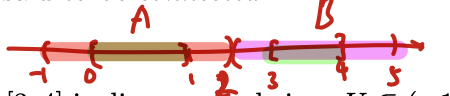
\includegraphics[width=\columnwidth]{images/disconnected.png}

\textbf{Theorem} A subset $E$ of $\mathbb{R}$ is connected iff $E$ is an interval.

\textbf{Theorem (Preservation of connectedness)} Let $f: S \mapsto \mathbb{R}$ be a continuous function. If $E$ is a connected subset of $S$, then $f(E)$ is connected.

\textbf{Corollary (Generalised form of preservation of closed intervals).} Let $f: S \mapsto \mathbb{R}$ be a continuous function. If $K$ is a connected compact subset of $S$, then $f(K) = [\inf f(K), \sup f(K)]$, a closed bounded interval.

\subsection{Calculus}
\textbf{L'Hospital's Rule.} Suppose that we have one of the following cases,

$$
\underset{x \mapsto \alpha}{\lim} \frac{f(x)}{g(x)} = \frac{0}{0} \text{ OR } \frac{\pm \infty}{\m \infty}
$$

where $\alpha$ can be any real number, $\pm \infty$. In these cases, we have,

$$
\underset{x \mapsto \alpha}{\lim} \frac{f(x)}{g(x)} = \underset{x \maps to \alpha}{\lim} \frac{f'(x)}{g'(x)}
$$

\textbf{Partial Fraction Decomposition.}
(1) Factor the bottom. $\frac{5x-4}{x^2 -x - 2} = \frac{5x-4}{(x-2)(x+1)}$.

(2) Write one partial fraction for each of those factors. $\frac{5x-4}{(x-2)(x+1)} = \frac{A_1}{x-2} + \frac{A_2}{x+1}$. 

(3) Multiply through by the bottom so we no longer have fractions. $5x - 4 = A_1 (x+1) + A_2 (x-2)$.

(4) Now find constants $A_1$ and $A_2$ by substituting the roots (i.e. $x = -1, 2$).

\textbf{Inequalities}

(i) \textbf{Multiplicative Inverse} If $a < b$, then $\frac{1}{ a} < \frac{1}{b}$

(ii) \textbf{Square Root Property} If $a \leq b$, then $\sqrt{a} \leq \sqrt{b}$

(iii) \textbf{Exponential} $f(x) = a^x$ is monotonely increasing/decreasing for $a > 1$ and $0 < a < 1$ respectively.

\textbf{$\sin$ properties}

(i) $\sin x \leq x$

(ii) $\sin x - \sin y = \sin \frac{x - y}{2} \cos \frac{x - y}{2}$

% \textbf{Exponential rules}

% $$
% \begin{aligned} a^{-1} &=1 / a \\\left(a^{m}\right)^{n} &=a^{m n} \\ a^{m} a^{n} &=a^{m+n} \\ e^{x} & \geq 1+x \end{aligned}
% $$

% \textbf{Log rules}

% $$
% \begin{aligned} a &=b^{\log _{b} a} \\ 
% \log _{c}(a b) &=\log _{c} a+\log _{c} b \\
% \log _{b} a^{n} &=n \log _{b} a \\
% \log _{b} a &=\frac{\log _{c} a}{\log _{c} b} \\
% \log _{b}(1 / a) &=-\log _{b} a \\
% \log _{b} a &=\frac{1}{\log _{a} b} \\
% a^{\log _{b} c} &=c^{\log _{b} a} \\
% e^{ln(x)} &= x \\
% loglog(n) &\neq (log^2n = (logn)^2)
% \end{aligned}
% $$

\subsection{List of Questions}

\textbf{The Real Numbers}

Define Bernoulli's Inequality.

Define Triangle Inequality and it's two corrollaries.

\textbf{The Completeness Property of $\mathbb{R}$}

Define $\epsilon-$neighborhood of $a$.

Define $\sup$ and $\inf$ and $sup/inf$ property.

Define Archimedean Property and corollary.

Define Density theorem (both rational and irrational).

Describe nested interval property.

How to prove convergence and calculate limits: five ways to identify limits (for cauchy criterion, state negation too).

Define divergent properties.

State relation between limits of subsequences and sequences (2).

State and define five ways to test if infinite series converge/diverge

\textbf{State and define three ways to test for absolute convergence.}

State relation between limit of modulus and modulus of limit

\textbf{Limits}

Define cluster point.

State ways to prove limits of functions (3, excluding one-sided limit)

State lower bound theorem.

\textbf{Continuous Functions}

State ways to show that a function is continuous at a point (4)

Define continuous functions and sequential criterion for continuity. State usefulness of relation to limit.

State discontinuity criterion.

State combinations/composition of functions.

% State boundedness theorem.

State max-min theorem.

State location of roots and intermediate value theorem.

Define preservation of closed intervals theorem.

How to prove uniform continuity (4)?

How to prove non-uniform continuity (2)?

Define theorems of uniform continuity (2x)

Define one-sided limits for monotone function exist theorem and it's usefulness.

Define jump and it's usefulness.

Define discontinuous points of monotone functions theorem.

Define continuous inverse theorem.

State usefulness of rational power functions.

\textbf{A glimpse into topology}

Define neighbourhood, open set, \textbf{closed set.}

Define open set properties, closed set properties.

Define characterisation of \textbf{closed sets} and open sets.

Define Global Continuity Theorem corollary

Define metric conditions

Define open cover

State intuitive understanding of disconnected

State theorems related to compactness (x2) and connectedness (x2)

State Generalised form of preservation of closed intervals

\textbf{Calculus}

What to do when you see $\frac{2n + 1}{n^2 (n+1)^2}$?

If $x < y$ and $0 < a < 1$, what's the inequality relating $a^x$ and $a^y$?

\subsection{Examples to relook}
2.1.13 (1, 2), 2.2.6(b), 2.4.1(b), 3.1.6(d), 3.2.8 (e), 3.4.3(a), 3.5.6(c), 3.7.6(c), T3Q2 (FD), T3Q5, T5Q2(a), T6Q3, 18/19 (Q2), 13/14(Q1(a), Q5(ii))

% 2.1.13 (1, 2), 2.2.6(b), 2.2.9(a), 2.4.1(i), Archimedean Property Proof, 2.4.2(a, c), 3.1.11, 3.16, 3.2.8 (b, f), Proof for T3.2.2, Proof for T3.2.3, 3.3.3(a), 3.3.4(a), 3.4.3 (a), 3.4.6(c), 3.5.2 (a,b), 

\vfill
\hrule
~\\
Prepared by Larry, AY2020/2021 Semester 1
\end{multicols}

\end{document} 